\chapter{Implementation}
Each unit is described by the following procedure:
\begin{itemize}
\item Overall design and block description - Quick design overview
\item Block breakdown - Detailed design overview
\item Block construction - Detailed implementation and calculations.
\end{itemize}
This procedure is meant to ease readability and help give an overview of the entire system implementation.
\section{CDU}

\section{Sensor Node}
The sensor node responsibility is, as described in the previous documents, to capture a temperature and support the custom powerline communication protocol. Below is described in detail how each block in the sensor node is implemented and designed.

\subsection{Overall design}
Below is shown a figure of the overall sensor node design.
\begin{figure}
\centering
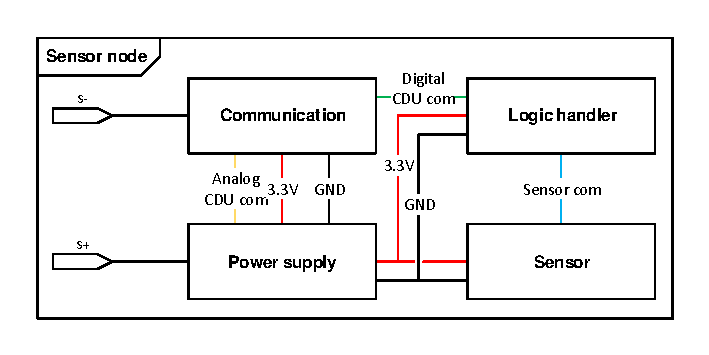
\includegraphics[width=.9\textwidth]{billeder/sn_overall_design}
\caption{Sensor node overall design}
\end{figure}

\subsubsection{Block description}
\textbf{Power supply:}\\
The power supply is creates a steady 3.3V supply to the system from the powerline communication bus.\\

\textbf{Communication:}\\
The communication block convertes the analog communication signal from the CDU to a digital stream of data and clock to the system and the digital communication from the logic handler to an analog signal on the bus to the CDU.\\

\textbf{Logic handler:}\\
The logic handler serves to analyse the incoming data transmission and act accordingly, at the current state this is to either respond with information about the sensor or respond with measured data.\\

\textbf{Sensor:}\\
The sensor part of the sensor node serves as the actual measurement circuit. This has a logical interface to the logic handler.\\

\subsection{Block breakdown}
This section describes the interfaces and the design of each individual block.\\
Below, in figure \ref{fig:SN_detailed} is shown a detailed overview of the sensor node design. This will be the basis of the block breakdown section.

\begin{figure}[H]
	\centering
	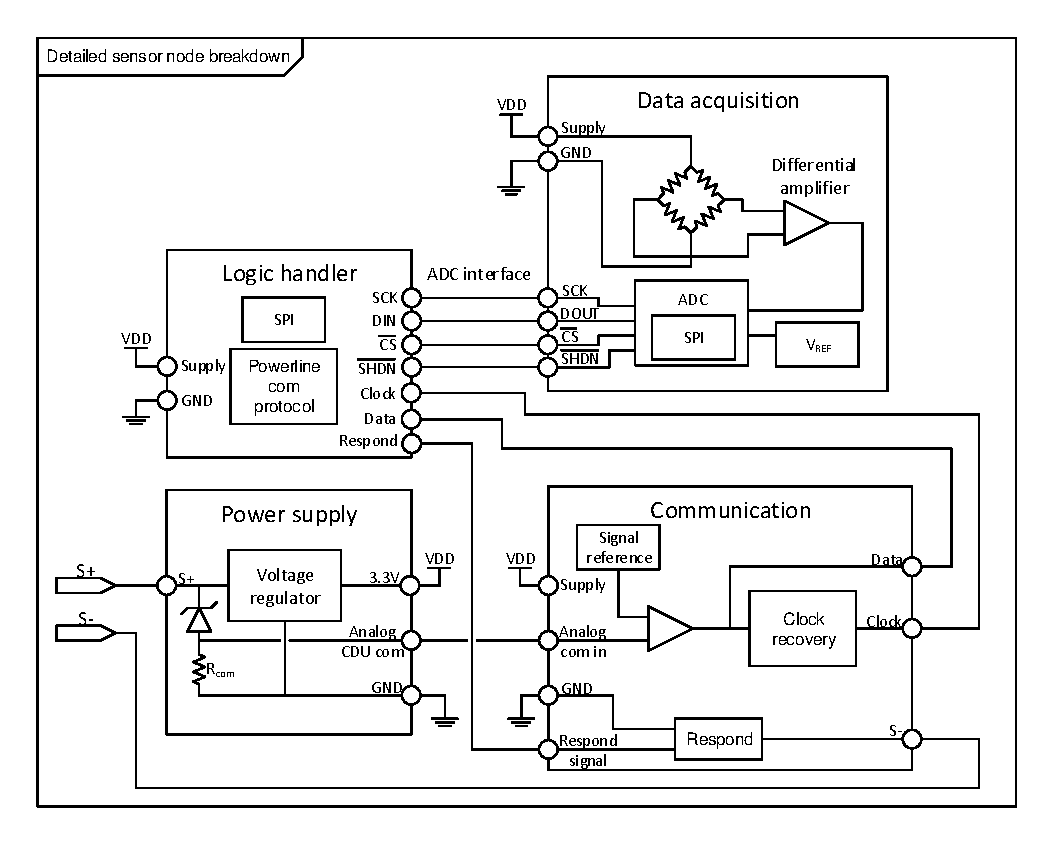
\includegraphics[width=1\textwidth]{billeder/SN_detailed_design}
	\caption{Detailed sensor node breakdown}
	\label{fig:SN_detailed}
\end{figure}

The following subsection will cover all interfaces and design considerations.

\subsubsection{Powersupply}
The power supply block is responsible for power to the entire sensor. This involves making 3.3V to the system in the sensor node and thereby making a reference voltage as ground to the system. Below in figure \ref{fig:SN_PS_FIGURE} is shown the interface to the power supply.

\begin{figure}[H]
	\centering
	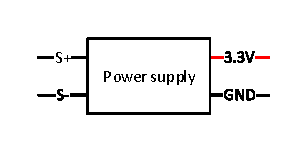
\includegraphics[width=.4\textwidth]{billeder/sn_powersupply_figure}
	\caption{Sensor node power supply block interfaces}
	\label{fig:SN_PS_FIGURE}
\end{figure} 

The goal is to create a steady 3.3V power to the components on the sensor node. The bus is specified as a line where all sensor nodes are placed in series. Therefore each sensor node has an individual reference ground. The line is a constant current modulated with communication.\\
Interface levels:
\begin{table}[H]
	\centering
	\begin{tabular}{|p{3cm} | p{3cm} | p{5cm}| }
		\hline
		Interface name: & 	Levels 								& Description \\ \hline
		S+ 				& 	$\geq$4.7V (with respect to GND) 	& The S+ input is the positive connection from the CDU. \\ \hline
		3.3V			&	3.3V (with respect to GND)			& This is the 3.3V supply voltage to the descrete components on the sensor node. \\ 	\hline
		Analog CDU com  &   $\sim$0V to $\sim$17.5mV			& The voltage drop caused by the communication current over the \\ \hline
		GND				&	0V									& Voltage reference ground on the individual sensor.\\\hline 
	\end{tabular}
\end{table}

The S+ and S- signals are from the powerline bus where S+ is connected to the previous sensor or the CDU B+ pin. The S- is connected to the next sensor or the CDU B- pin.\\
Below, on figure \ref{fig:SN_detailed_ps}, is shown a simplified implementation of the powersupply.

\begin{figure}[H]
	\centering
	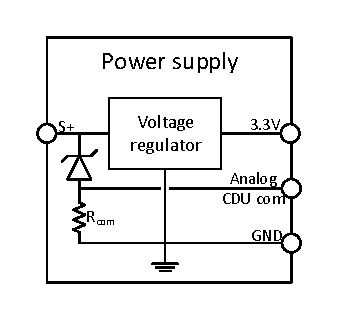
\includegraphics[width=.5\textwidth]{billeder/powersupply_detailed_sn}
	\caption{Detailed powersupply design.}
	\label{fig:SN_detailed_ps}
\end{figure}

The diode and R$_{\text{com}}$ creates a voltage drop from which the voltage regulator creates the steady 3.3V suuply. The R$_{\text{com}}$ resistor serves to "convert" the current modulated communication to a voltage to the communication block.

\subsubsection{Communication}
The communication block generates a steady synchronized clock and converts data to the correct logic levels. It also has a logical interface which enables responds to the CDU by modulate the current drop over the entire sensor. Below in figure \ref{fig:SN_com_fig} the communication block interfaces is shown.

\begin{figure}[H]
	\centering
	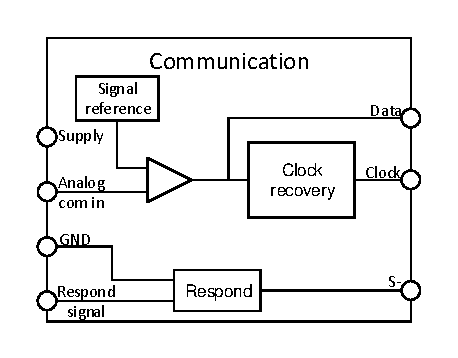
\includegraphics[width=.5\textwidth]{billeder/communication_sn}
	\caption{Sensor node communication block interfaces}
	\label{fig:SN_com_fig}
\end{figure}

The purpose of the communication is to synchronize the sensor node clock to the CDU clock to make sure the data is sampled properly.

\begin{table}[H]
	\centering
	\begin{tabular}{|p{3cm} | p{3cm} | p{5cm}| }
		\hline
		Interface name: & 	Levels 								& Description \\ \hline
		Supply			& 	3.3V							 	& 3.3V from the power supply. \\ \hline
		Analog com in	&	$\sim$0V to $\sim$17.5mV 			& The voltage-converted communication signal from the CDU.\\ \hline
		Respond signal  &   $\sim$0V to $\sim$3.3V				& Digital input with the respond to the CDU from the logic handler. \\ \hline
		GND				&	0V									& Voltage reference ground on the individual sensor.\\\hline 
	\end{tabular}
\end{table}


\subsubsection{Logic handler}

\subsubsection{Sensor}